\section{Discussion \& Limitations}
\label{sec:discussion}

%\wajih{Use macros for common words in this whole section.}

%\wajih{Be consistent with the terminology that you used in the abstract/intro.}

%\wajih{Move adversarial attacks in a separate section.}

%% \PP{Adversarial Attacks Analysis} We discussed robustness to mimicry attacks in Section~\ref{sec:mimicry}. Here, we address vulnerabilities to other types of adversarial attacks, including gradient-based attacks, model poisoning, and inference attacks (discussed in Section~\ref{sec:privacy}). Addressing these attacks is beyond the scope of this paper, as we focus on establishing an end-to-end framework for privacy-aware PIDS. We plan to integrate advancements in adversarial defense mechanisms against such attacks into \Sys to enhance its robustness in future work. These integrations are discussed below.

% Gradient-based adversarial attacks~\cite{chakraborty2021survey} typically require white-box access to the target machine learning model, including its parameters. This necessity often renders them impractical for real-world applications. In contrast, black-box attacks, which utilize iterative, query-based techniques, tend to be more detectable and complex to implement due to their conspicuous nature. Such attacks are feasible if an attacker manages to compromise a client machine. However, during the operational phase, a compromised client cannot affect other clients because they are working independently. Several existing defenses can be employed during model training to enhance the system's resilience against these attacks. Adversarial training~\cite{tramer2019adversarial} is one effective strategy, wherein the model is trained with perturbed input data to increase its robustness to such attacks.

% During the training phase, poisoning attacks executed by malicious actors may introduce corrupt weights to compromise the global model~\cite{jagielski2018manipulating}. To improve \Sys's resilience against such threats, several defensive methods can be used. Among these, advanced model aggregation methods, such as Multi-Krum~\cite{munoz2019byzantine}, can be particularly effective. This method employs clustering techniques on the central server to identify anomalous updates during model aggregation. Consequently, outlier updates are removed, enhancing the system's robustness against poisoning.

\subsection{RQ4: Adversarial Attacks Analysis}
\label{sec:adversarial}

% \wajih{would it be possible to combine Figure 4 and Figure 3 into one figure with three subflots/subfigures.}

% \begin{figure}[!t]
%   \centering
%   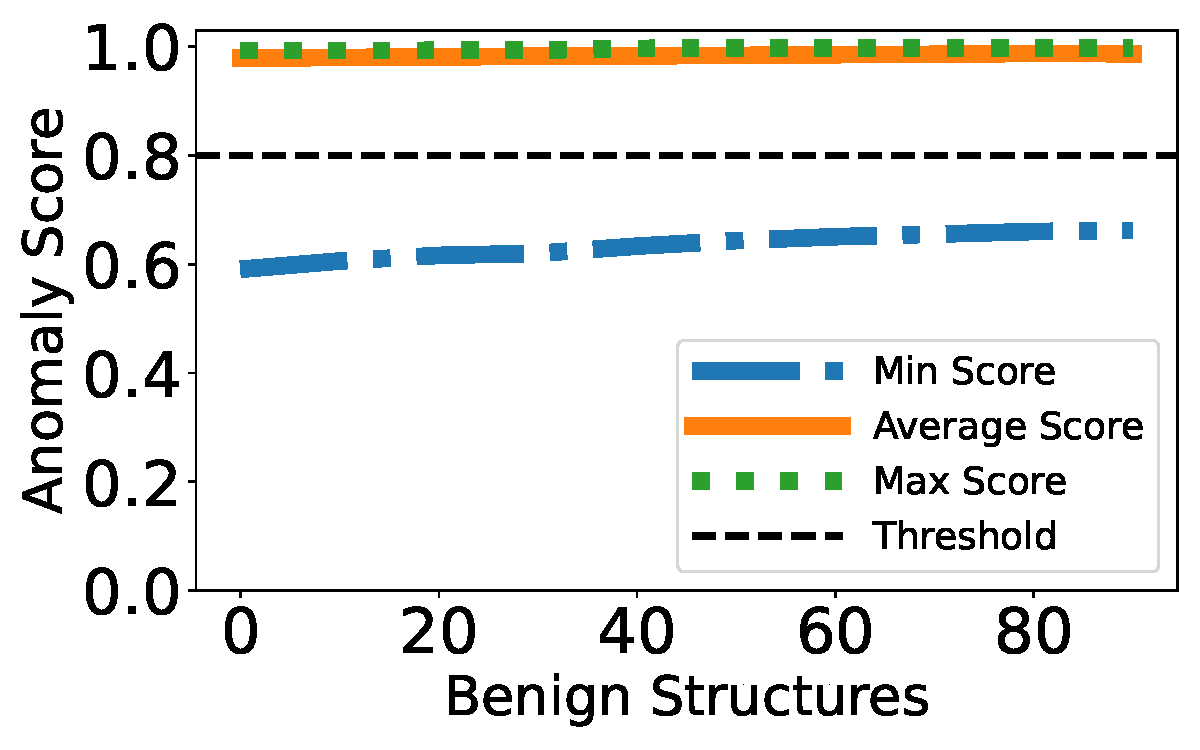
\includegraphics[width=0.34\textwidth]{fig/adversarial.pdf}
%   \caption{Adversarial mimicry attack analysis.}
%   \label{mimicryattack}
%   \vspace{-2ex}
% \end{figure}


In this section, we analyze the robustness of our system against mimicry, model poisoning, gradient-based attacks and bin-level inference attacks. Membership inference attacks are discussed in Section~\ref{sec:privacy}.

\begin{figure*}[!t]
  \centering
  \subfloat[Model poisoning: FedAvg aggregation.]{%
    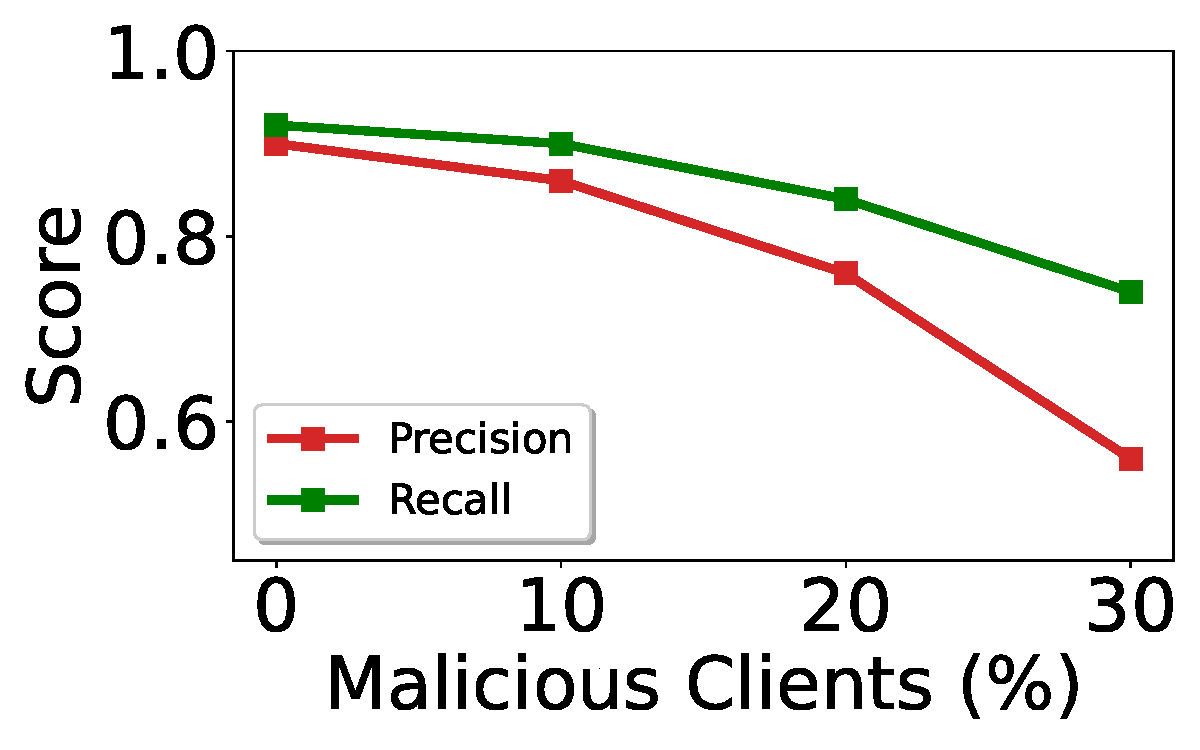
\includegraphics[height=0.15\textwidth]{fig/FedAvg_poisoning.pdf}%
    \label{fedavgpoison}
  }
  \hfill
  \subfloat[Model poisoning: Multi-Krum aggregation.]{%
    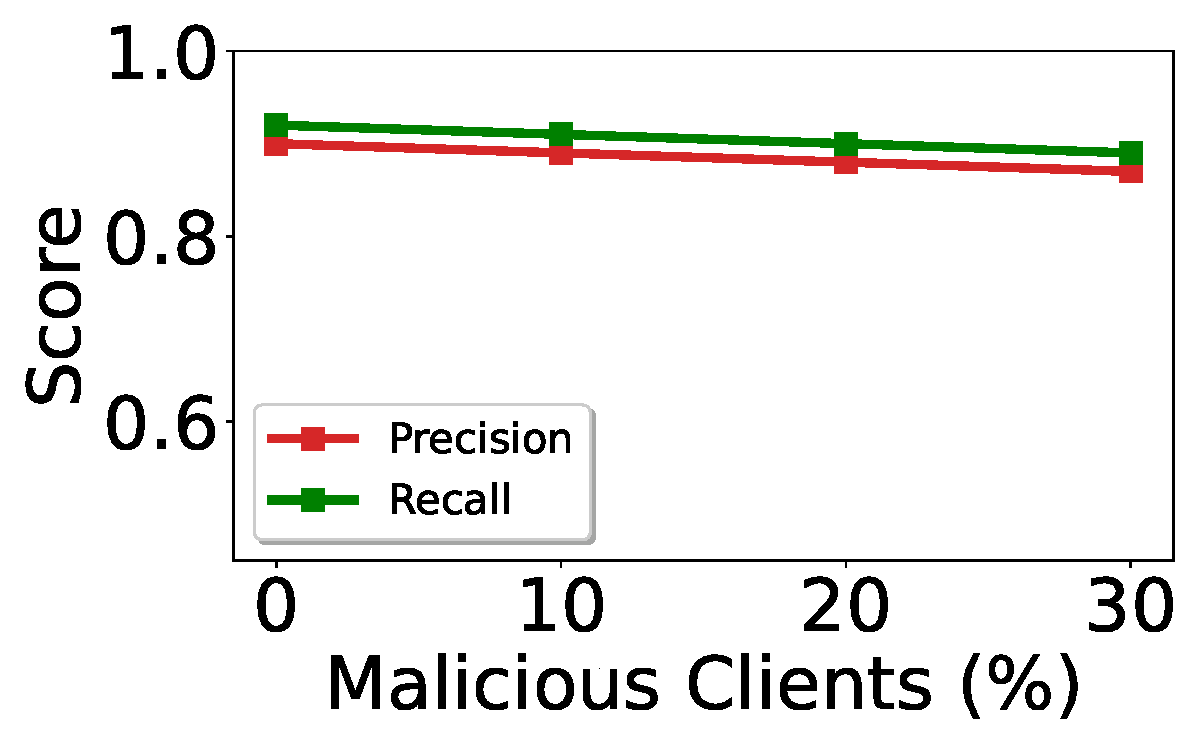
\includegraphics[height=0.15\textwidth]{fig/multi-krum.pdf}%
    \label{multikrumpoison}
  }
  \hfill
  \subfloat[Adversarial mimicry attack]{%
    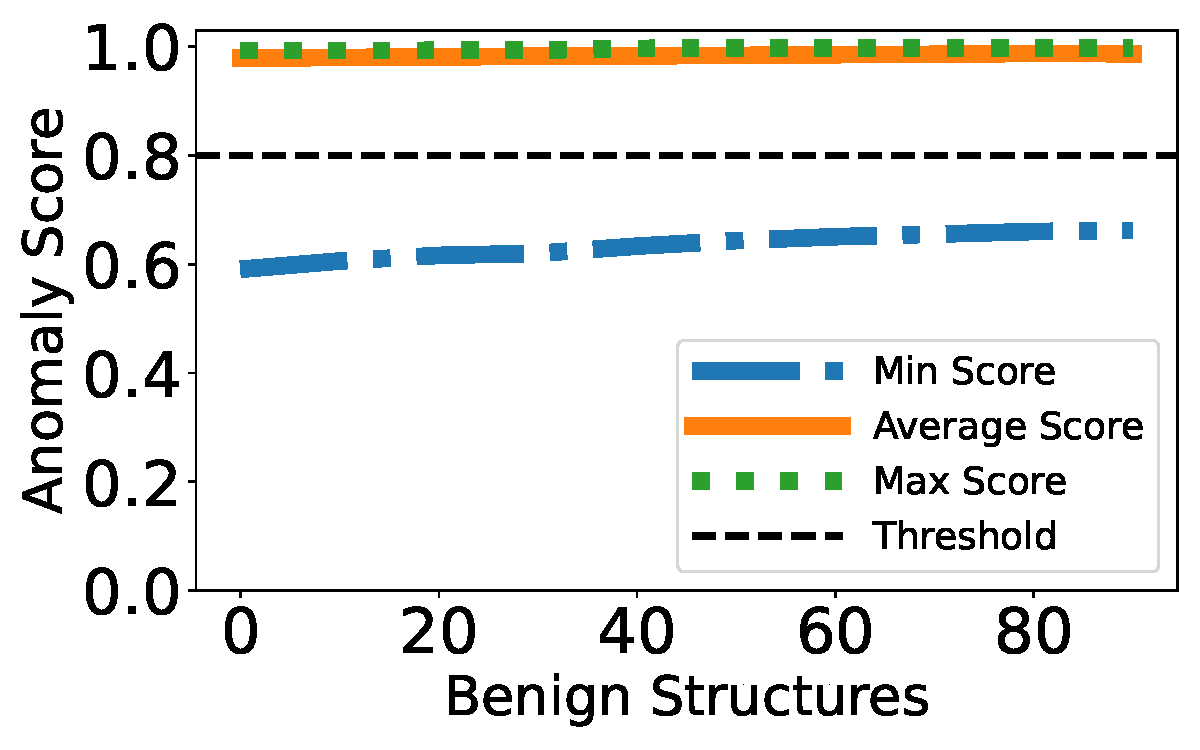
\includegraphics[height=0.15\textwidth]{fig/adversarial.pdf}%
    \label{mimicryattack}
  }
  \hfill
  \caption{Adversarial attacks analysis.}
  \label{fig:poison}
  \vspace{-3ex}
\end{figure*}

\PP{Mimicry Attacks}  We evaluated our system's resilience against the adversarial mimicry attack detailed by Goyal et al.~\cite{goyal2023sometimes} and compared its robustness with \flash. The attack aims to mimic benign graph embeddings, integrating benign node structures to evade detection. Using the E3 dataset, similar to \flash for fair comparison, our findings (shown in Figure~\ref{mimicryattack}) reveal that our detector remains robust; the integration of benign structures has a minimal impact on anomaly scores. Our system's superior robustness is due to our process-categorization-based ensemble \gnnshort architecture, which allows model specialization for different system entities, enhancing detection of structural changes. Conversely, \flash, relying on a generalized model for anomaly detection, exhibits vulnerabilities to mimicry attacks, as it may miss critical details. As demonstrated by the authors, \flash initially experiences a drop in anomaly scores, increasing the likelihood of attack nodes evading detection which is a vulnerability not present in our system. \footnote{PROVNINJA~\cite{mukherjee2023evading} is another mimicry attack that uses benign process profiles to find adversarial evasion strategies. It faces challenges against \pids like \flash and \Sys due to their multimodal architecture, which combines \wordvec for featurization and \gnnshort for anomaly detection. This complexity makes it difficult for attackers to create effective evasion strategies without accessing \wordvec directly or excessively querying the model, which conflicts with the black box nature of the assumed threat model of PROVNINJA.}


\PP{Model Poisoning Attacks} These occur when one or more malicious clients submit corrupted local model updates to the central server during training, thereby degrading the model’s performance. Existing methods typically assume an attack-free training phase, providing no defense against such attacks. We conducted experiments on the \optc dataset to assess the impact of poisoning attacks on our system, and we also evaluated how robust aggregation methods, such as Multi-Krum~\cite{munoz2019byzantine}, can enhance resilience.

Multi-Krum compares each client’s gradient with those of other clients, retaining only the most consistent updates. Since malicious updates must deviate significantly from benign ones to degrade performance, Multi-Krum effectively identifies and discards them as outliers. Figure~\ref{fig:poison} shows our experimental results using both FedAvg and Multi-Krum. With simple federated averaging, malicious noise critically affects the model by disrupting the benign distribution it learns. In contrast, Multi-Krum isolates and removes erroneous updates from malicious clients, preserving the global model. Notably, Multi-Krum assumes that fewer than one-third of all clients are malicious; therefore, in our experiments, we tested with a maximum of 30\% compromised clients.



\PP{Gradient-based Attacks} These attacks~\cite{chakraborty2021survey} exploit detailed knowledge of the target model, including its architecture and parameters, to calculate and apply malicious perturbations. Such white-box access allows an attacker to compute precise gradients that indicate how inputs should be modified to degrade the model’s performance. Other attacks tend to be black-box in nature, relying on iterative, query-based techniques to influence the model’s decisions. However, these repeated computations and queries run counter to the attacker’s aim of remaining inconspicuous, as they generate substantial activity and leave a significant footprint. Consequently, such attacks are often impractical in real-world scenarios. Several defenses can be employed during model training to bolster the system’s resilience against these threats. Adversarial training~\cite{tramer2019adversarial} is one effective strategy in which the model is trained on perturbed input data, thereby increasing its robustness against these attacks.

\PP{Bin-level Inference Attacks}  
In addition to the privacy risks outlined in Section~\ref{sec:privacy}, we identify another potential avenue for information leakage: bin-level inference attacks during training. In this scenario, a malicious client attempts to infer information about system entities held by other clients. It does so by manipulating the tokens it submits and observing changes in the utility server's harmonized vectors. Since overlapping token vectors are averaged, any noticeable change in the returned vector indicates that the token is shared across clients within the organization.  However, unlike the central and utility server inference risks, this attack does not compromise client identities and only the presence of a token in the system is revealed, preserving anonymity. Furthermore, our threat model~\ref{sec:threat}, consistent with prior \pids works, assumes a benign training environment free from adversarial clients. Bin-level inference attacks are thus only feasible during the training-time harmonization phase and not during deployment. We leave the development of federated learning methods robust to such adversarial training settings as an important direction for future work.


\PP{Combining FL with \gnnshort} APTs involve multiple causally linked attack steps across system entities, requiring provenance graphs to effectively model these interactions. Existing log-level systems~\cite{deeplog2017,liu2019log2vec,xia2019loggan} fail to capture such interactions, while graph representation learning excels at identifying patterns in these graphs~\cite{flash2024,cheng2023kairos,jia2023magic}. By integrating federated learning with graph representation learning, \Sys enables privacy-preserving, decentralized intrusion detection without compromising detection performance.

\PP{Alert Investigation} Validating alerts in systems like \Sys is critical for reliability and avoiding alert fatigue~\cite{nodoze2019}. Traditionally, security analysts manually review alerts based on activities within local provenance graphs, but this process is time-consuming, error-prone, and lacks scalability and privacy. Privacy-preserving techniques such as Secure Multi-party Computation (SMC)~\cite{goldreich1998secure}, Homomorphic Encryption (HE)~\cite{yi2014homomorphic}, and Zero-Knowledge Proofs (ZKP)~\cite{fiege1987zero} can address these challenges. SMC enables collaborative alert validation while preserving input privacy, HE ensures confidentiality during encrypted data analysis, and ZKP allows one party to prove an alert's validity without revealing additional information. We identify privacy-preserving alert verification as a promising research direction. We leave it to future work to develop methods for privately sharing alert data with a central server, enabling security analysts to perform more in-depth attack analysis.

\PP{Explainability} Deep learning models used in \pids, including \Sys, function as black-box systems, making it challenging to interpret their decision-making processes. Like other \pids~\cite{flash2024,cheng2023kairos,yangprographer}, \Sys faces this interpretability issue, which hampers its adoption compared to rule-based systems. Existing explainability techniques~\cite{antwarg2021explaining,brown2018recurrent,ardito2021revisiting,hwang2021sfd} primarily focus on metrics like feature importance. However, modern \pids employ complex feature engineering, such as \flash's use of \wordvec for textual attribute processing and subsequent anomaly detection via \gnn models. This multi-model approach limits the applicability of existing explainable AI techniques. We identify explainable \pids as a critical area for future research. Recent advancements in LLMs~\cite{chang2024survey} offer potential solutions. Future research can leverage LLMs' reasoning capabilities to develop methods for interpreting \pids outputs effectively.


\PP{Log Retention} Effective log retention \cite{wilbert2012log,rapsheet2020} is essential for \pids performance and reliability, particularly for investigating APTs that span months. Decentralized systems like \Sys and \disdet store raw logs on client machines with limited storage, constraining retention periods based on the deployment domain. To address this, \Sys can integrate secure, tamper-resistant cloud storage solutions~\cite{kumar2018secure,hardlog} for backing up logs. During attack investigations, logs related to alerts raised by \Sys can be retrieved, processed to remove sensitive attributes for privacy preservation \cite{portillo2019towards}, and used for detailed analysis.

\PP{Concept Drift} Concept drift occurs when the data distribution of the system evolves over time, potentially invalidating the patterns learned by \Sys during training. Emerging system activities can result in new benign behaviors being misclassified as anomalies. To address this, periodic retraining with recent data is essential to update the models. Strategies from recent works~\cite{lu2018learning, barbero2022transcending,jordaney2017transcend} provide effective approaches for mitigating concept drift.

% \PP{State Explosion in Massive Networks} Scaling FL to larger enterprise networks introduces potential state explosion issues, primarily due to the increasing complexity in managing and integrating updates from a growing number of clients. As more clients participate, each contributing their local model updates, the volume of data to be processed and aggregated can increase significantly. This escalation can strain communication channels, leading to higher bandwidth requirements and increased latency. Furthermore, the aggregation process itself becomes more computationally demanding as the number of updates grows. \Sys addresses these challenges by utilizing an ensemble learning approach and categorizing system activities, which simplifies the aggregation by processing more uniform data segments. Moreover, our system uses models with small network overhead to prevent bandwidth challenges. To further enhance efficiency, additional techniques such as model compression~\cite{choudhary2020comprehensive}, selective update aggregation~\cite{ye2020federated} and the implementation of more robust communication protocols~\cite{laclau2020robust} can significantly improve handling large volumes of updates, thus preventing state explosion and maintaining system performance in large-scale federated learning environments.

\PP{Unseen Tokens in Semantic Encoder} \Sys relies on \wordvec models to encode semantic attributes, but \wordvec only generates embeddings for tokens it has previously encountered, which can degrade the quality of feature vectors for new nodes with unseen tokens. To construct node representations, we combine semantic attributes with neighboring nodes' system calls, but for nodes with unseen tokens, the representation is predominantly based on system calls, as seen in systems like \threatrace~\cite{wang2022threatrace}. To address this limitation, retraining the \wordvec model more frequently or adopting subword-level embedding models like fastText~\cite{joulin2016bag}, which generate embeddings from subword units, can improve coverage. Tokenization methods such as Byte-Pair Encoding~\cite{araabi2022effective} further enhance new token representation by breaking unknown words into smaller subword components.



% \wajih{add citations for different techniques (SMC, HE, etc.) below}

%\PP{Retraining Frequency} \wajih{Discuss here how often we need to retrain models on client machines. You can say that it depends on enterprise settings, in our experiments we found that XXX times per day gave us good results.}

%\wajih{Investigation using \Sys. We need to add one paragraph saying something about how to do an investigation using \Sys after detection. It does not have to be detailed. We just need to show that we thought about this problem. At the end of the paragraph say that we leave this for future work.}

%\wajih{Talk about why we did not consider other privacy-preserving techniques beyond the federation, such as secure multi-party computation or homomorphic encryption.}